\section{Lagrangian Regions}
\label{sec:lagrangianregions}

\subsection{Definition of a Lagrangian Region}

\begin{figure}
    \centering
    \includegraphics[width=\columnwidth]{figures/lagrangian_region_high_mass_mnras.pdf}
    \caption{The lagrangian region associated with a $7\times10^{13}$
	$\mathrm{M}_\odot$ halo at $z=0$, shown in the inset plot. The local
	particle density in this region is approximately constant; the
	structure shown here is due to the particle selection, rather than any
	real structure in the overall distribution. Colour encodes projected
	denisity.}
    \label{fig:lrpic}
\end{figure}

A lagrangian region is defined as the region in the initial conditions where
the dark matter from a given collapsed object at lower redshift resides. This
definition is somewhat open to interpretation; there may be particles enclosed
in the convex hull of such a region that do not end up in the collapsed object,
especially in an incorrect choice is made for the gravitational softening. The
following discussion describes comparison with redshift $z=0$ compact objects
but this definition is easily extensible to higher redshift.

To determine the collapsed objects at $z=0$ the AMIGA halo finder
\citep[AHF][]{ahfi, ahfii} is used. This spherical overdensity finder
determines the halo centers by using a nested grid, and then fits parameters
based on the Nevarro-Frenk-White \citep[NFW, ][]{nfw} profile.

It is impractical, especially considering the nature of this paper, to use the
baryonic matter resident in a collapsed object to define the appropriate
`baryonic' lagrangian region. Instead, a nearest neighbour search for each gas
particle at $z=z_{\rm ini}$ is performed and each particle assigned a
lagrangian region identifier that corresponds to that of the nearest dark
matter particle. This ensures that the two regions overlap very tightly
spatially, which is important when considering the very fine-grained detail
present in these regions (see Figure \ref{fig:lrpic}).

As noted previously, there was a bug in the simulation code that prevents gas
particles that have formed stars, and star particles that have been formed
out of gas particles which have already formed a star, from being included in
this analysis.

\subsection{Matching Lagrangian IDs}

Each dark matter particle in the simulation is assigned, based on the known
unique particle ID, a largangian region identifier that cooresponds to the halo
ID of the associated $z=0$ collapsed object. Particles which end up outside of
any halo at $z=0$ are assigned a lagrangian region identifier of -1. Once this
has been performed, the gas particles may be matched as described above, with
the nearest neighbour search. Once all particles in the initial conditions have
been assigned a lagrangian region, they must be ID matched with particles in
the final $z=0$ snapshot of the simulation. This is performed by looping
through all of the (sorted) particles and assigning a lagrangian region ID for
the final-state particles that is equal to that of their initial state
progenitor. To assign a largrangian region to the star particles at $z=0$,
their gas progenitor (which can be tracked using the unique particle ID) is
used. Particles which either become black holes, or are consumed by a black
hole, are ignored for this analysis. This re-matching also takes place for the
dark matter particles, to ensure that the ID matching is working correctly.

\subsection{Quantifying Inter-Lagrangian Transfer}

\begin{figure} \centering
	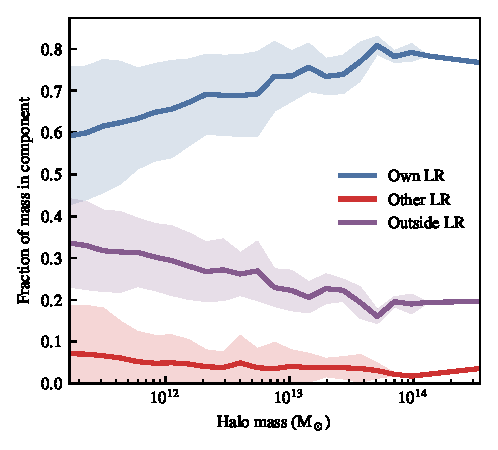
\includegraphics[width=\columnwidth]{generated_figures/component_fraction_vs_halo_mass_both.pdf}
	\caption{The fraction of total baryonic mass in a given halo at $z=0$
	as a function of halo mass. These values are computed using the
	lagrangian region IDs that were assigned to the gas and star particles
	in the initial conditions. See Figure \ref{fig:splitmassfrac} for a
	breakdown into stellar and gaseous components. The shaded regions show
	a single standard deviation of variance in the mass fraction for that
	bin, and do not include errors from halo sampling bias or cosmic
	variabnce.} \label{fig:massfrac} \end{figure}

Once this analysis has been performed it is possible to see the fraction of
baryonic mass at $z=0$ that originates from the lagrangian region of a given
halo (see Figure \ref{fig:massfrac}). There is a significant difference in the
contributions from the gaseous and stellar components to this mass fraction;
see Figure \ref{fig:splitmassfrac}. This data is for every halo in the box, and
hence does not include any cuts based on the particlar neighbourhood of these
halos; a significant fraction of the scatter here is likely to come from
isolated halos, versus those in clusters and other noisier environments. This
analyis shows that a significant portion (up to 20\%) of the stellar mass of a
Milky-Way mass halo may come from the lagrangian region as defined by a
\emph{different halo}.

\begin{figure*} \centering
	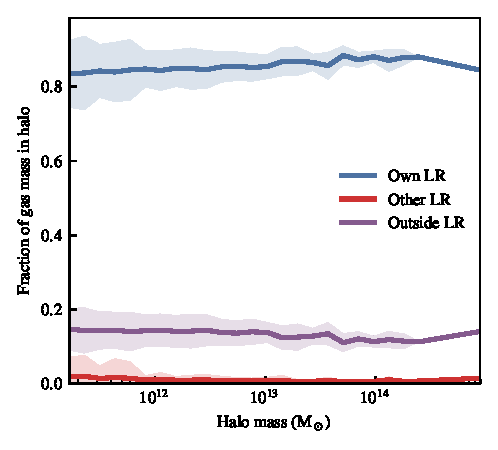
\includegraphics[width=0.495\textwidth]{generated_figures/component_fraction_vs_halo_mass_gas.pdf}
	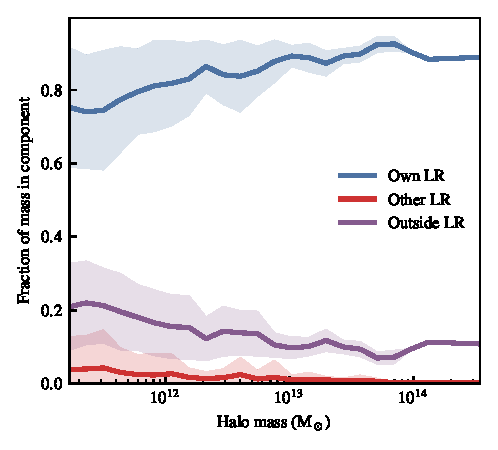
\includegraphics[width=0.495\textwidth]{generated_figures/component_fraction_vs_halo_mass_stellar.pdf}
	\caption{Left: fraction of gaseous mass at $z=0$ in each halo from each
	component; right: fraction of stellar mass at $z=0$ from each
	component. Note that there is significantly more transfer shown in the
	gaseous component. Gas that is transferred between lagrangian regions
	must be given time to cool before being able to form stars. As the
	events that enable transfer are typically very energetic (AGN, stellar
	feedback, accretion), it is unlikely that the cooling time will be
	short enough to form stars by the end of the simulation for most
	transfer.} \label{fig:splitmassfrac} \end{figure*}

It is important to note that this spread in mass fractions as a function of
halo mass is still to be quantified. It could be that those halos which
end up having less mass transfer are those which are more isolated; in future
analysis we hope to include the isolation criteria used in, for example, the
APOSTLE project \citep{fattahi2016} to select halos and compare their mass
fractions. This inter-lagrangian transfer could have a significant effect
on these high-resolution zoom-in galaxies that is not correctly captured
using the current isolation criteria.

\subsection{Radial Trends}

\begin{figure} \centering
	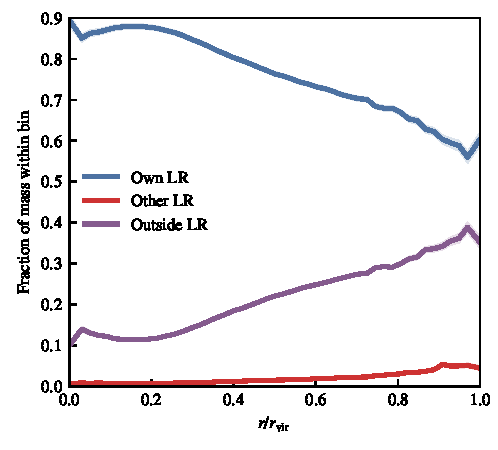
\includegraphics[width=\columnwidth]{generated_figures/radial_distance_plot.pdf}
	\caption{The dependence of mass fraction split by component as a
	function of radius, normalised by the virial radius for each halo.
	Every halo with $10^{12} \leq $ M$_{\rm halo}$ $ < 10^{13}$ M$_\odot$
	is stacked in this plot, with the shaded regions giving standard errors
	around the mean. Solid lines show the trends for gas, with the dashed
	lines showing the same but for the stellar component of the halo. 50
	bins were spaced linearly in radius.} \label{fig:radialmassfrac}
\end{figure}

The mass fractions contributed from various components to each halo appear to
be relatively independent of halo mass (see Figure \ref{fig:massfrac}), however
this may not be true within each individual halo. In Figure
\ref{fig:radialmassfrac} the mass fraction contributed to the halo is shown as
a function of radius. As expected, more gas in the center of the halo comes
from the corresponding lagrangian region, but interestingly this only
approaches ~60\%, suggesting significant transfer \emph{into halos} still takes
place for gas that ends up at the bottom of the potential well at $z=0$.

Also note how the mass fraction of stars from the own lagrangian region of the
halo drops as a function of radius. This suggests that a large number ($\sim{}30$\%)
of these stars were formed ex-situ. Note, again, that around $\sim{}$15\% of the stars
at the center of these halos are formed from gas that was not present in the
initial lagrangian region of this halo. This is surprising, as this transfer
must have taken place relatively early to ensure that the gas was able to cool
and form stars.

These radial trends tell us something about the assembley of the
Circum-Galactic Medium (CGM) \citep{tumlinson2017}. Whilst the claim can be
that the \simba{} simulation suite does not have the requisite resolution to
accurately simulate the CGM, these trends are very tight and show strong
convergence when multiple halos are stacked.  \citet{Crain2013} found that the
CGM assmembles from the `inside-out', with feedback within the galaxy
establishing a strong negative metallicity relation.  However, these results
seem to suggest there is a significant effect from inter-lagrangian (and hence
inter-galactic) transfer from gas that has been blown out of \emph{other}
galaxies falling in to add to this metallicity gradient.  Future work will
focus on separating these two variables using this analysis.
